\documentclass[12pt,a4paper]{report}

% ------------------------------------------------------------
% Packages
% ------------------------------------------------------------
\usepackage[a4paper,margin=0.9in]{geometry}
\usepackage{graphicx}
\usepackage{amsmath,amssymb}
\usepackage{booktabs}
\usepackage{array}
\usepackage{tabularx}
\usepackage{longtable}
\usepackage{float}
\usepackage{caption}
\usepackage{setspace}
\usepackage{enumitem}
\usepackage{hyperref}
\usepackage{url}
\usepackage{fancyhdr}

\hypersetup{
    hidelinks,
    pdftitle={3D Ship Battle Simulation Using OpenGL},
    pdfauthor={Tawhidul Hasan}
}

\graphicspath{{figures/}{report/figures/}}
\setstretch{1.06}
\setlength{\parindent}{0.30in}
\setlength{\parskip}{0.08em}
\setlist[itemize]{itemsep=0.10em, topsep=0.20em}
\setlist[enumerate]{itemsep=0.10em, topsep=0.20em}

\pagestyle{fancy}
\fancyhf{}
\fancyhead[L]{3D Ship Battle Simulation Using OpenGL}
\fancyhead[R]{\thepage}
\renewcommand{\headrulewidth}{0.4pt}
\setlength{\headheight}{15pt}

\newcommand{\code}[1]{\texttt{\detokenize{#1}}}
\newcommand{\reportfilename}[1]{\texttt{\detokenize{#1}}}
\newcolumntype{Y}{>{\raggedright\arraybackslash}X}

% Compact figure macro. Real images are also limited in height so the
% report stays within the page limit after screenshots are added.
\newcommand{\placeholderfigure}[3]{%
\begin{figure}[H]
    \centering
    \IfFileExists{#1}{%
        \includegraphics[width=0.82\textwidth,height=0.21\textheight,keepaspectratio]{#1}%
    }{%
        \fbox{%
        \parbox[c][34mm][c]{0.78\textwidth}{%
            \centering\small
            Insert project screenshot here\\[1mm]
            \reportfilename{#1}%
        }}%
    }
    \caption{#2}
    \label{#3}
\end{figure}}

\begin{document}

% ============================================================
% COVER PAGE
% ============================================================
\begin{titlepage}
    \thispagestyle{empty}
    \centering

    \vspace{0.6cm}
    {\LARGE\bfseries 3D Ship Battle Simulation Using OpenGL\par}

    \vspace{2.3cm}
    {\large\textbf{Submitted by:}\par}
    \vspace{0.35cm}
    {\Large Tawhidul Hasan (2107004)\par}

    \vspace{1.8cm}
    {\large\textbf{Submitted to:}\par}
    \vspace{0.45cm}
    {\large\textbf{Md Tajmilur Rahman}, Lecturer\par}
    \vspace{0.18cm}
    {\large\textbf{Md. Mubtashim Abrar Nihal}, Lecturer\par}

    
    \vspace{2.8cm}
    
     % KUET logo. Keep kuet-logo.png in the same Overleaf folder as main.tex.
    \IfFileExists{kuet-logo.png}{%
        \includegraphics[width=5.2cm]{kuet-logo.png}%
    }{%
        \fbox{\parbox[c][2.8cm][c]{5.2cm}{\centering KUET LOGO}}%
    }

    \vfill
    {\large Department of Computer Science and Engineering\par}
    \vspace{0.12cm}
    {\large Khulna University of Engineering \& Technology\par}
    \vspace{0.12cm}
    {\large Khulna 9203, Bangladesh\par}
    \vspace{0.40cm}
    {\large 10 October, 2026\par}
    \vspace*{0.7cm}
\end{titlepage}

% ============================================================
% FRONT MATTER
% ============================================================
\pagenumbering{roman}
\setcounter{page}{1}

\chapter*{Abstract}
\addcontentsline{toc}{chapter}{Abstract}
This project presents a real-time 3D ship battle simulation made with C++ and OpenGL. Its main goal is to demonstrate important computer graphics topics in one interactive scene. The program includes a controllable ship, enemy ships, cannon fire, animated water, lighting, weather, camera control, particles, ports, missions, and other world objects.

OpenGL is used for rendering, GLFW for the window and input, GLAD for loading OpenGL functions, and GLM for vector and matrix operations. The project demonstrates translation, rotation, scaling, hierarchical transformations, camera matrices, Flat shading, Gouraud shading, Phong shading, and time-based animation. It also contains a genuine hybrid ray-tracing pass: rasterization draws the scene while each visible ocean fragment can trace a sun-visibility ray against a bounded analytic proxy scene. The project is designed as a graphics demonstration rather than a physically exact naval simulator.

\tableofcontents
\clearpage

\pagenumbering{arabic}
\setcounter{page}{1}

% ============================================================
% CHAPTER 1
% ============================================================
\chapter{Introduction}

\section{Project Overview}
The project is titled \emph{3D Ship Battle Simulation Using OpenGL}. The basic idea is to create a real-time naval scene where ships move on the sea and fire cannons. The project is mainly used to demonstrate 3D transformations, animation, lighting, shading, camera movement, and user interaction. The original proposal is treated as a project requirement document rather than cited as an external academic authority.

The final program extends the basic idea with ports, missions, weather, wildlife, crew activity, navigation, and several visual effects. The scene is rendered directly with OpenGL instead of using a game engine.

\placeholderfigure{figures/main_scene.png}{Main view of the 3D ship battle simulation.}{fig:main-scene}

\section{Problem Statement}
A ship battle scene combines many graphics problems. Ships must move and rotate correctly, the camera must follow the action, the water must look alive, and lighting must make the 3D shapes clear. Cannonballs and particles also need continuous animation.

The main challenge is therefore to combine these graphics techniques in one stable real-time application while keeping the implementation easy to understand.

\section{Objectives and Scope}
The main objectives are:
\begin{enumerate}
    \item Build an interactive 3D ship battle scene using C++ and OpenGL.
    \item Use translation, rotation, scaling, and hierarchical transformations correctly.
    \item Implement ambient, diffuse, and specular lighting.
    \item Demonstrate Flat, Gouraud, and Phong shading.
    \item Animate water, ships, cannonballs, particles, weather, and world objects.
    \item Provide keyboard and mouse controls for sailing, combat, camera movement, and graphics options.
\end{enumerate}

The project focuses on real-time computer graphics. It is not intended to be a physically exact naval simulator. Some objects and effects are simplified so the program remains suitable for a course project and runs in real time.

\section{Authorship}
The submitted project and report identify Tawhidul Hasan (Roll 2107004) as the sole student author. Accordingly, the implementation responsibilities in this report are not divided among unverified team members. The source history and supplied documents should be used if a later submission needs a more detailed chronological contribution statement.

\section{Main Tools and Libraries}
\begin{table}[H]
\centering
\caption{Main tools and libraries used in the project.}
\label{tab:tools}
\begin{tabularx}{0.92\textwidth}{>{\bfseries}p{0.20\textwidth}Y}
\toprule
Tool / Library & Purpose \\
\midrule
C++17 & Main programming language. \\
OpenGL 3.3 Core & Renders the 3D scene. \\
GLFW & Creates the window and handles input. \\
GLAD & Loads OpenGL functions. \\
GLM & Provides vectors, matrices, and transformations. \\
GLSL & Implements vertex and fragment shaders. \\
CMake & Builds and organizes the project. \\
\bottomrule
\end{tabularx}
\end{table}

\clearpage
\section{Proposed and Implemented Feature Comparison}
The original two-page proposal described a small continuously running naval battle containing a sea surface, two or more procedurally constructed ships, movable cannons, visible cannonballs, a simple sky, a directional light, Phong illumination, transformation composition, continuous animation, and optional keyboard control. Table~\ref{tab:proposal-audit} compares those statements with the inspected final source. ``Extended'' means the proposed capability is present and the final implementation goes materially beyond its original scope.

\begin{longtable}{p{0.22\textwidth}p{0.13\textwidth}p{0.55\textwidth}}
\caption{Original proposal compared with the final implementation.}\label{tab:proposal-audit}\\
\toprule
\textbf{Proposed feature} & \textbf{Status} & \textbf{Evidence in the final project} \\
\midrule
\endfirsthead
\toprule
\textbf{Proposed feature} & \textbf{Status} & \textbf{Evidence in the final project} \\
\midrule
\endhead
Sea surface & Extended & \code{Waves.h} defines four travelling wave components; \code{basic.vert} displaces the ocean and derives its normal; \code{basic.frag} adds foam, shoreline colour, Fresnel blending, and an underwater surface. \\
Two or more ships & Extended & The player and combat enemy use full hierarchical ships. \code{LivingWorld.h} adds routed pirate, merchant, naval, and neutral traffic with distance-based representations. \\
Ship and cannon motion & Extended & The ship has delta-time translation and steering, wave-driven heave/pitch/roll, sail states, an anchor, wheel and rudder motion, cannon aiming, recoil, and broadside batteries. \\
Visible cannonball flight & Fully implemented & A bounded array of 96 projectiles is updated using velocity and gravity. Water, land, ship, mast, rail, and explosive-keg impacts produce different outcomes. \\
Simple procedural models & Extended & \code{Ship.h}, \code{Hull.h}, and \code{Planks.h} build the galleon procedurally. Ports, scenery, wildlife, cargo, interiors, and effects also reuse generated meshes and OpenGL transformations. \\
Directional lighting and Phong model & Fully implemented & \code{Lighting.h} contains the shared ambient, diffuse, specular, attenuation, material, and emission calculations. Daylight and moonlight occupy the directional-light slot. \\
Transformations and composition & Fully implemented & GLM model, view, projection, and normal matrices are uploaded to GLSL. Parent frames store rigid transforms while object scale is applied only at the draw call. \\
Continuous animation & Extended & The main loop uses measured and clamped \(\Delta t\). Ships, crew, cargo work, wildlife, particles, projectiles, weather transitions, and camera motion update continuously. \\
Keyboard interaction & Extended & Sailing, firing, ammunition, sails, anchor, cameras, map, trading, environment, shading modes, lighting terms, ray tracing, HUD, and debugging are all interactive. \\
Additional final systems & Beyond proposal & Ports, cargo economy, ten linked missions, treasure clues, a world chart, underwater exploration, below-deck rooms, damage/fire/explosions, factions, persistent discoveries, and hybrid ray-traced ocean shadows were added after the proposal. \\
\bottomrule
\end{longtable}

This comparison avoids treating every late-stage idea as part of the original promise. The original scope is fully represented; the larger world systems are identified as extensions and remain deliberately simplified where a full commercial simulation would require physics, content tools, or external assets.

% ============================================================
% CHAPTER 2
% ============================================================
\chapter{Graphics Concepts and Design}

\section{System Architecture}
The program uses one central \code{SceneState} in \code{main.cpp}. It owns the current camera, ships, combat state, environment, particles, crew, campaign, living world, and UI flags. CPU-only headers calculate state and transforms; drawing headers convert that state into calls to the shared mesh renderer. This separation allows campaign logic, collision checks, dolphin continuity, enemy routing, and ray--sphere mathematics to be tested without creating an OpenGL context.

\begin{table}[H]
\centering
\caption{Major modules and their responsibilities.}
\label{tab:architecture}
\small
\begin{tabularx}{0.97\textwidth}{p{0.22\textwidth}p{0.25\textwidth}Y}
\toprule
\textbf{Module} & \textbf{Important types/functions} & \textbf{Responsibility} \\
\midrule
\code{main.cpp} & \code{SceneState}, \code{processInput}, \code{updateScene}, \code{renderScene} & Owns the frame loop and synchronizes all subsystems. \\
\code{Ship.h} & \code{ShipPose}, \code{ShipFrames} & Produces the rigid parent--child frame hierarchy for hull, decks, masts, yards, sails, and weapons. \\
\code{Lighting.h} & \code{computeLighting}, \code{lightContribution} & Supplies one GLSL lighting implementation to both shader stages so Gouraud and Phong differ only in evaluation stage. \\
\code{Waves.h} & \code{waterSurfaceY}, wave GLSL source & Keeps CPU ship motion and GPU ocean displacement based on the same wave parameters. \\
\code{Particles.h}, \code{Fx.h} & \code{ParticleSystem}, \code{DamageSystem}, \code{ExplosionSystem} & Maintains bounded particles, damage states, fire, explosions, debris, sails, anchor, steering, and ship AI helpers. \\
\code{Campaign.h} & \code{CampaignSystem}, \code{PortSystem}, \code{CargoSystem}, \code{NavigationSystem} & Stores missions, docking, trading, cargo, port NPCs, treasure-map state, and chart navigation. \\
\code{LivingWorld.h} & \code{LivingWorldSystem}, \code{WorldVessel} & Generates regions, routed traffic, factions, encounters, discoveries, and persistent world state. \\
\code{Interior.h} & \code{InteriorLayout}, \code{Explorer} & Defines the hold rooms, furniture, colliders, ladders, chests, and on-foot movement. \\
\code{basic.vert/.frag} & vertex and fragment stages & Performs transformations, ocean displacement, shading selection, water composition, and hybrid sun-shadow rays. \\
\bottomrule
\end{tabularx}
\end{table}

The frame dependency is
\begin{equation}
\text{events}\rightarrow\text{input state}\rightarrow\text{simulation}(\Delta t)
\rightarrow\text{world transforms}\rightarrow\text{draws}\rightarrow\text{HUD}\rightarrow\text{swap}.
\end{equation}
Temporary OpenGL state is restored by each specialized pass. For example, the ocean temporarily disables face culling and enables its reflection blend, then restores culling, disables blending, and resets \code{uSeaMode}. This prevents water rendering from changing later ship and world draws.

\section{Rendering Pipeline and Transformations}
The program follows the normal OpenGL rendering process. In each frame, it reads input, updates the scene, transforms the 3D objects, renders them, and displays the final image \cite{foley,openglref,glsl}. In simple form:
\begin{equation}
\text{Input} \rightarrow \text{Update} \rightarrow \text{Transform} \rightarrow \text{Render} \rightarrow \text{Display}.
\end{equation}

Each object starts in local coordinates. A model matrix places it in the world:
\begin{equation}
\mathbf{M}=\mathbf{T}\mathbf{R}\mathbf{S},
\end{equation}
where \(\mathbf{T}\) is translation, \(\mathbf{R}\) is rotation, and \(\mathbf{S}\) is scaling. A point is then transformed by
\begin{equation}
\mathbf{p}_{clip}=\mathbf{P}\mathbf{V}\mathbf{M}\mathbf{p}_{local},
\end{equation}
where \(\mathbf{V}\) is the camera view matrix and \(\mathbf{P}\) is the perspective projection matrix. GLM is used to build these matrices \cite{glm}.

The ship uses hierarchical transformations. Parts such as masts, sails, cannons, and crew are placed relative to the main ship. When the ship moves or turns, these parts follow it automatically.

For a translation \((t_x,t_y,t_z)\) and non-uniform scale \((s_x,s_y,s_z)\), GLM constructs the homogeneous matrices
\begin{equation}
\mathbf{T}=\begin{bmatrix}1&0&0&t_x\\0&1&0&t_y\\0&0&1&t_z\\0&0&0&1\end{bmatrix},\qquad
\mathbf{S}=\begin{bmatrix}s_x&0&0&0\\0&s_y&0&0\\0&0&s_z&0\\0&0&0&1\end{bmatrix}.
\end{equation}
For example, heading is a rotation about the vertical axis:
\begin{equation}
\mathbf{R}_y(\theta)=\begin{bmatrix}
\cos\theta&0&\sin\theta&0\\0&1&0&0\\-\sin\theta&0&\cos\theta&0\\0&0&0&1
\end{bmatrix}.
\end{equation}
Matrix order is significant because column vectors are used. A child point is evaluated as \(\mathbf{M}_{parent}\mathbf{M}_{local}\mathbf{p}\); therefore the local operation occurs first. The code intentionally keeps scale out of stored parent frames, preventing a scaled deck from stretching a child mast. Surface normals use
\begin{equation}
\mathbf{N}_{world}=\operatorname{normalize}\!\left((\mathbf{M}_{3\times3}^{-1})^{T}\mathbf{N}_{local}\right),
\end{equation}
which is required when a model contains non-uniform scale.

\section{Camera System}
The project uses a perspective camera so distant objects appear smaller. Several camera modes are available, including chase or orbit views, free views, first-person-style views, and prepared camera positions. Mouse movement and scrolling can rotate or zoom supported views.

The perspective matrix maps a vertical field of view \(f_y\), aspect ratio \(a\), and near/far distances \(n,f\) into clip space. Its characteristic scale terms are \(1/(a\tan(f_y/2))\) horizontally and \(1/\tan(f_y/2)\) vertically. The view matrix is formed from the eye position, target direction, and world-up vector. Chase mode orbits a target attached to the player ship; free mode integrates motion along the current look direction; first-person, captain, and below-deck modes transform local eye positions through the ship hierarchy. Camera shake from explosions is added as a short decaying offset rather than changing the ship transform.

\section{Lighting and Shading}
The lighting system uses three common terms:
\begin{itemize}
    \item \textbf{Ambient light} gives a small amount of general light.
    \item \textbf{Diffuse light} becomes stronger when a surface faces the light.
    \item \textbf{Specular light} creates shiny highlights.
\end{itemize}

A material stores ambient, diffuse, and specular coefficients \(\mathbf{k}_a,\mathbf{k}_d,\mathbf{k}_s\), shininess \(n_s\), and optional emission \(\mathbf{k}_e\). The shared GLSL source in \code{Lighting.h} implements
\begin{equation}
\mathbf{I}_a=\mathbf{I}_{global}\odot\mathbf{k}_a,
\end{equation}
\begin{equation}
\mathbf{I}_d=a(d)\,\mathbf{I}_{L}\odot\mathbf{k}_d
\max(\mathbf{N}\cdot\mathbf{L},0),
\end{equation}
\begin{equation}
\mathbf{I}_s=a(d)\,\mathbf{I}_{L}\odot\mathbf{k}_s
\max(\mathbf{R}\cdot\mathbf{V},0)^{n_s},
\end{equation}
where \(\mathbf{N}\), \(\mathbf{L}\), \(\mathbf{V}\), and \(\mathbf{R}\) are normalized surface-normal, light, view, and reflected-light directions. The directional sun uses \(a(d)=1\). The point light uses
\begin{equation}
a(d)=\frac{1}{a_0+a_1d+a_2d^2}.
\end{equation}
The complete local model is
\begin{equation}
\mathbf{I}=\mathbf{I}_a+\sum_{j}\left(\mathbf{I}_{d,j}+\mathbf{I}_{s,j}\right)+\mathbf{k}_e.
\end{equation}
Ambient is evaluated once, outside the two-light loop. The \code{K} key isolates lighting terms; \code{L} changes the light mask; and \code{B} switches the specular test from Phong's \((\mathbf{R}\cdot\mathbf{V})^{n_s}\) to Blinn--Phong's \((\mathbf{N}\cdot\mathbf{H})^{n_s}\).

The program supports three shading modes. \textbf{Flat shading} uses one normal for a triangle, so polygon faces are easy to see. \textbf{Gouraud shading} calculates lighting at vertices and interpolates the colors across the triangle \cite{gouraud}. \textbf{Phong shading} interpolates the normal and calculates lighting for each fragment, which usually gives smoother highlights \cite{phong}.

For barycentric weights \(\lambda_0+\lambda_1+\lambda_2=1\), Gouraud shading interpolates completed vertex colours,
\begin{equation}
\mathbf{I}(p)=\lambda_0\mathbf{I}_0+\lambda_1\mathbf{I}_1+\lambda_2\mathbf{I}_2.
\end{equation}
Phong shading instead interpolates and renormalizes the normals,
\begin{equation}
\mathbf{N}(p)=\operatorname{normalize}(\lambda_0\mathbf{N}_0+\lambda_1\mathbf{N}_1+\lambda_2\mathbf{N}_2),
\end{equation}
then evaluates the same \code{computeLighting} function per fragment. This is why a narrow specular maximum between vertices can be absent in Gouraud shading but visible in Phong shading. The two modes share one shader program and one lighting source, so their comparison does not contain independently tuned equations.

\placeholderfigure{figures/gouraud_shading.png}{Scene rendered using Gouraud shading.}{fig:gouraud}
\placeholderfigure{figures/phong_shading.png}{The same scene rendered using Phong shading.}{fig:phong}

\section{Geometry, Water, and Environment}
The project reuses simple meshes such as cubes, cylinders, spheres, quads, grids, and triangles. Larger objects are built from these shapes. The ship, for example, contains a hull, decks, masts, sails, cannons, railings, anchor parts, and cargo. Reusing meshes saves memory and also demonstrates object construction through transformations.

The water surface uses several moving sine waves. A simplified wave equation is
\begin{equation}
h(x,z,t)=\sum_i A_i\sin\left(k_i(\mathbf{d}_i\cdot(x,z))-\omega_i t+\phi_i\right).
\end{equation}
Here, \(A_i\) controls wave height, \(\mathbf{d}_i\) controls direction, and time \(t\) moves the waves. The ship also uses the wave information so its movement matches the sea.

The environment changes sky color, haze, rain, wind, wave strength, and light intensity. Storm scenes use darker lighting, stronger waves, and rain. Night scenes use moonlight and brighter lantern effects.

\placeholderfigure{figures/ship_model.png}{Procedurally constructed ship model.}{fig:ship-model}

\clearpage
\section{Weather and Time-of-Day Rendering}
The environment is data driven. \code{Environment.h} defines fixed day, sunset, and night bases and five weather modifiers: sunny, cloudy, rainy, misty, and storm. \code{composeAtmosphere} combines the selected records into sun/moon direction and colour, global ambient light, horizon and zenith colours, haze density, cloud appearance, rain, wind, wetness, wave amplitude, foam, and lantern intensity. Transitions interpolate from the atmosphere currently shown to the target instead of changing every parameter in one frame. Dynamic mode derives sun motion and weather spells deterministically from the game clock.

\begin{figure}[H]
\centering
\begin{tabular}{ccc}
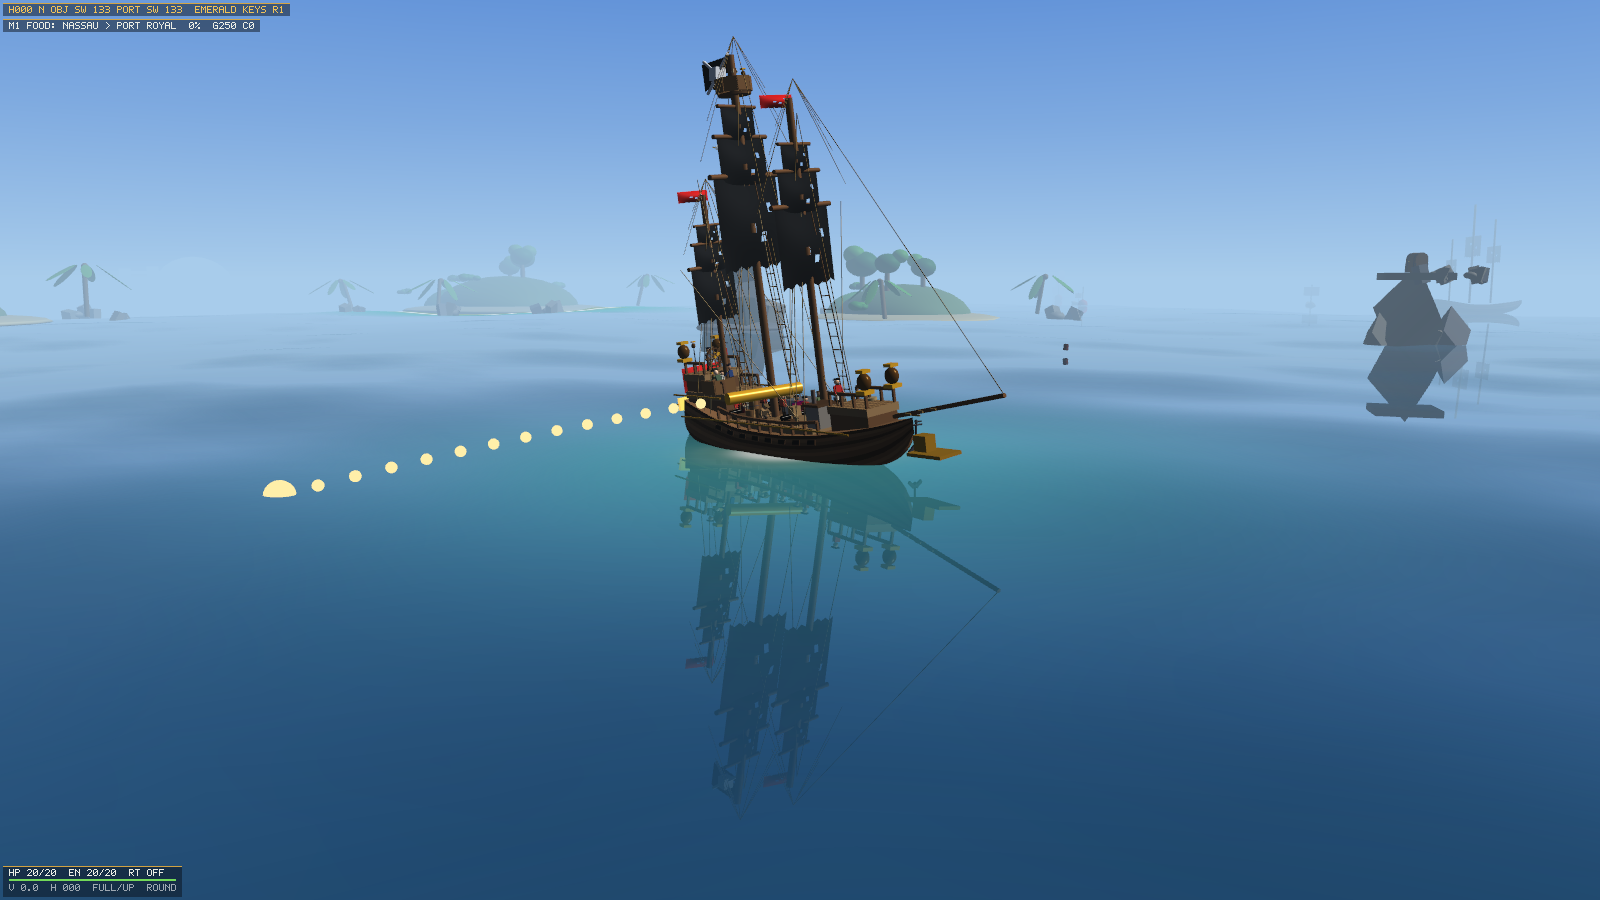
\includegraphics[width=0.31\textwidth]{figures/weather_sunny.png} &
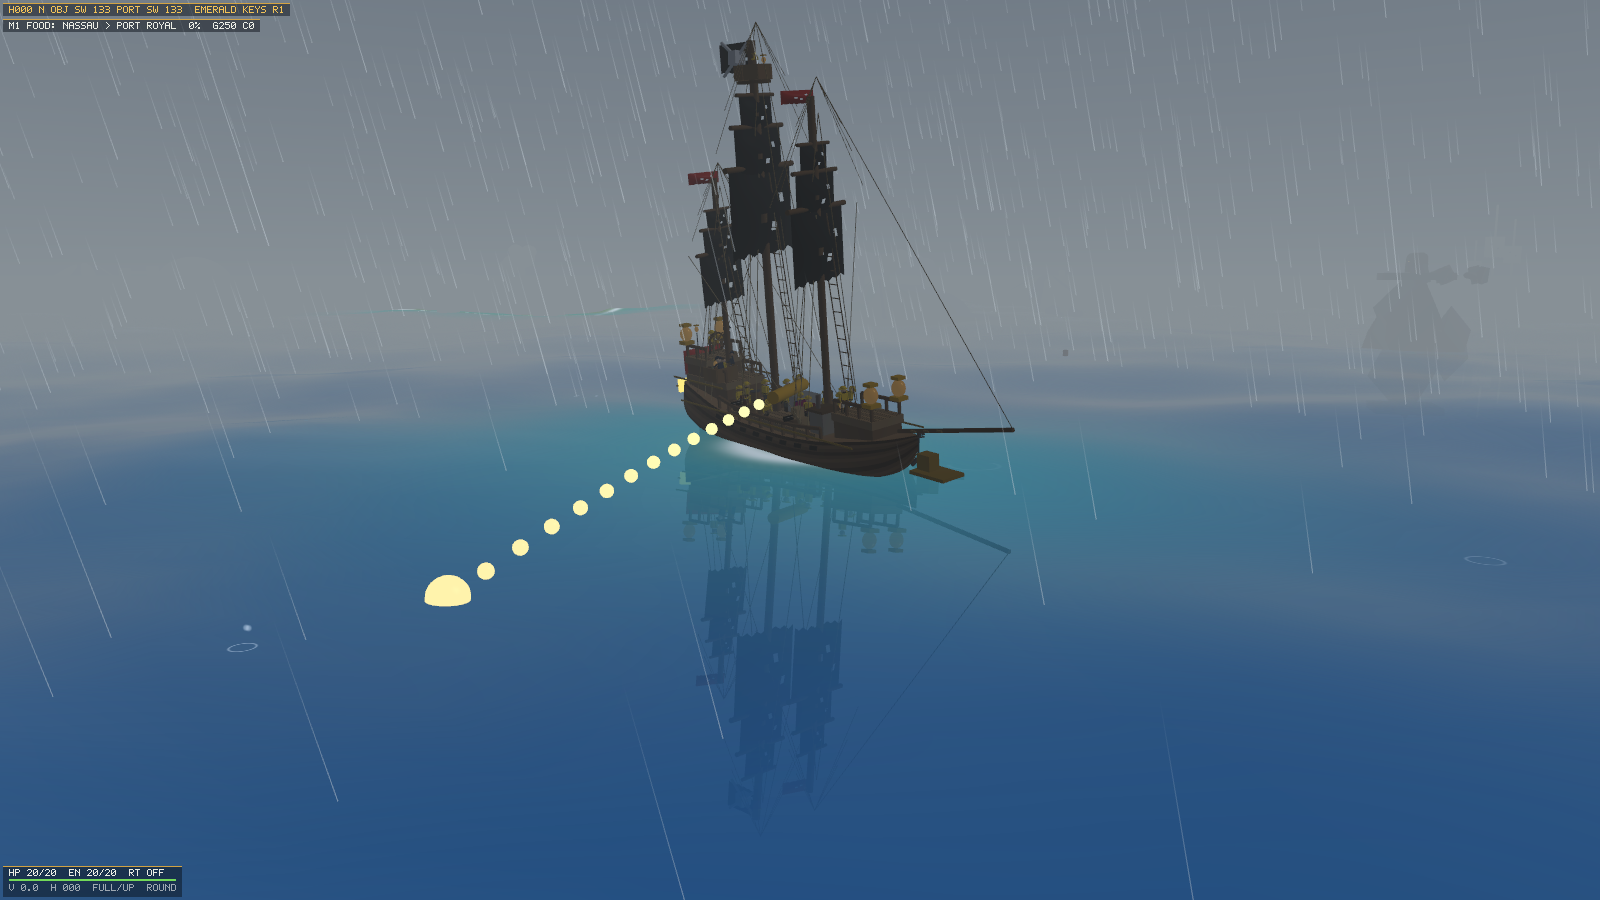
\includegraphics[width=0.31\textwidth]{figures/weather_rainy.png} &
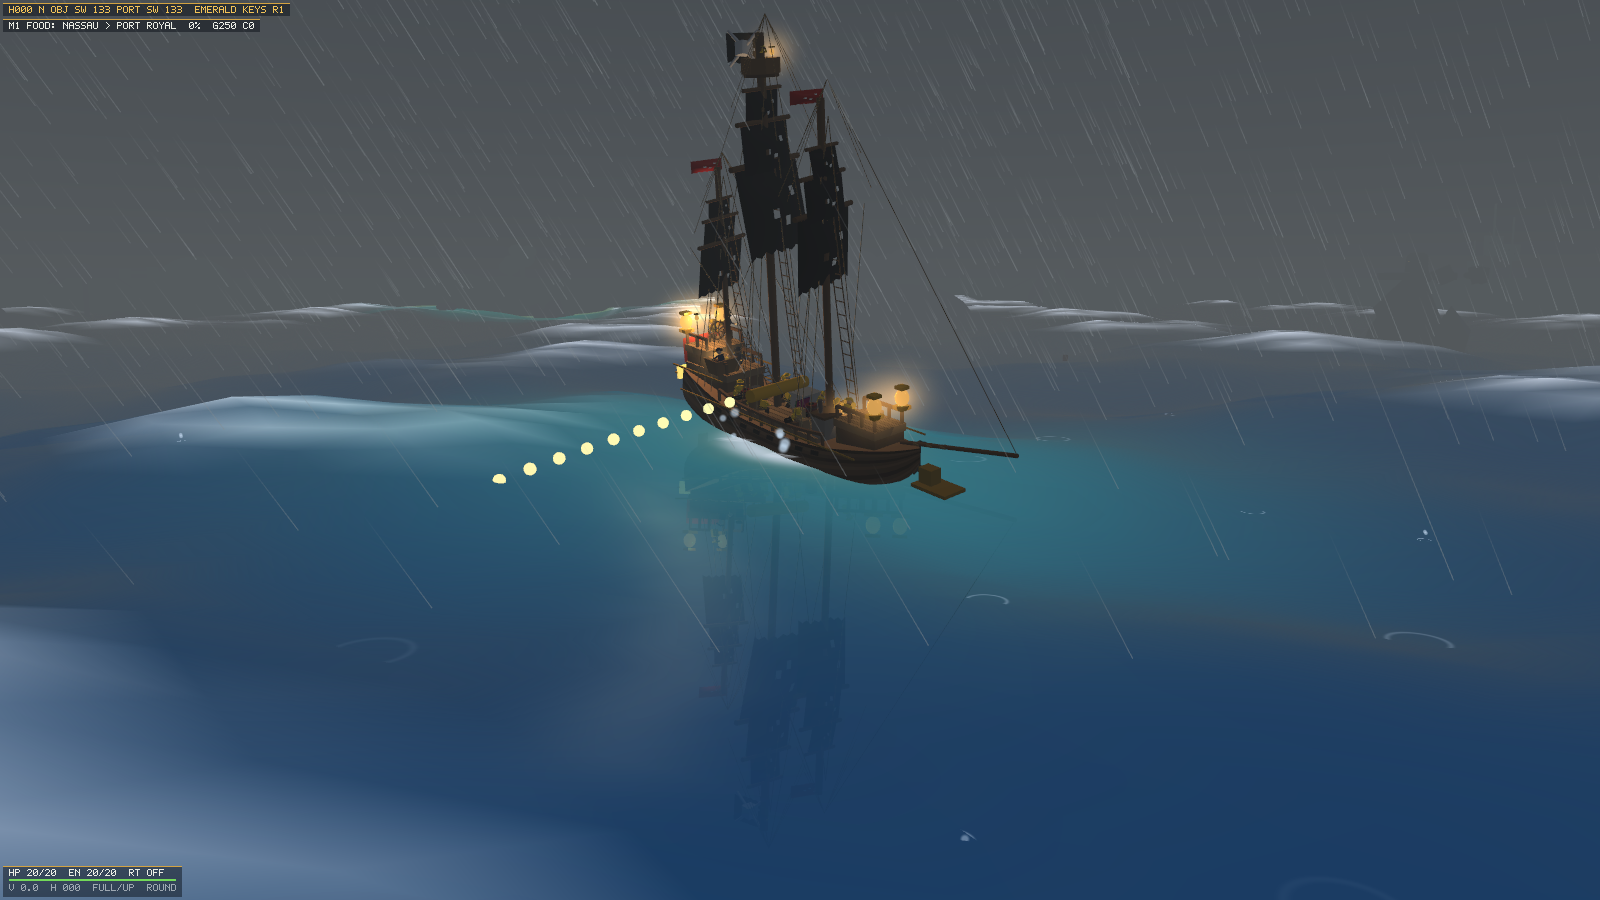
\includegraphics[width=0.31\textwidth]{figures/weather_storm.png} \\
\small Sunny & \small Rainy & \small Storm \\
\end{tabular}
\caption{Weather comparison from one location, time setting, and camera. Rain adds wind-driven line particles and wet materials; the storm also raises the wave scale, foam, darkness, and lightning response.}
\label{fig:weather-comparison}
\end{figure}

\begin{figure}[H]
\centering
\begin{tabular}{ccc}
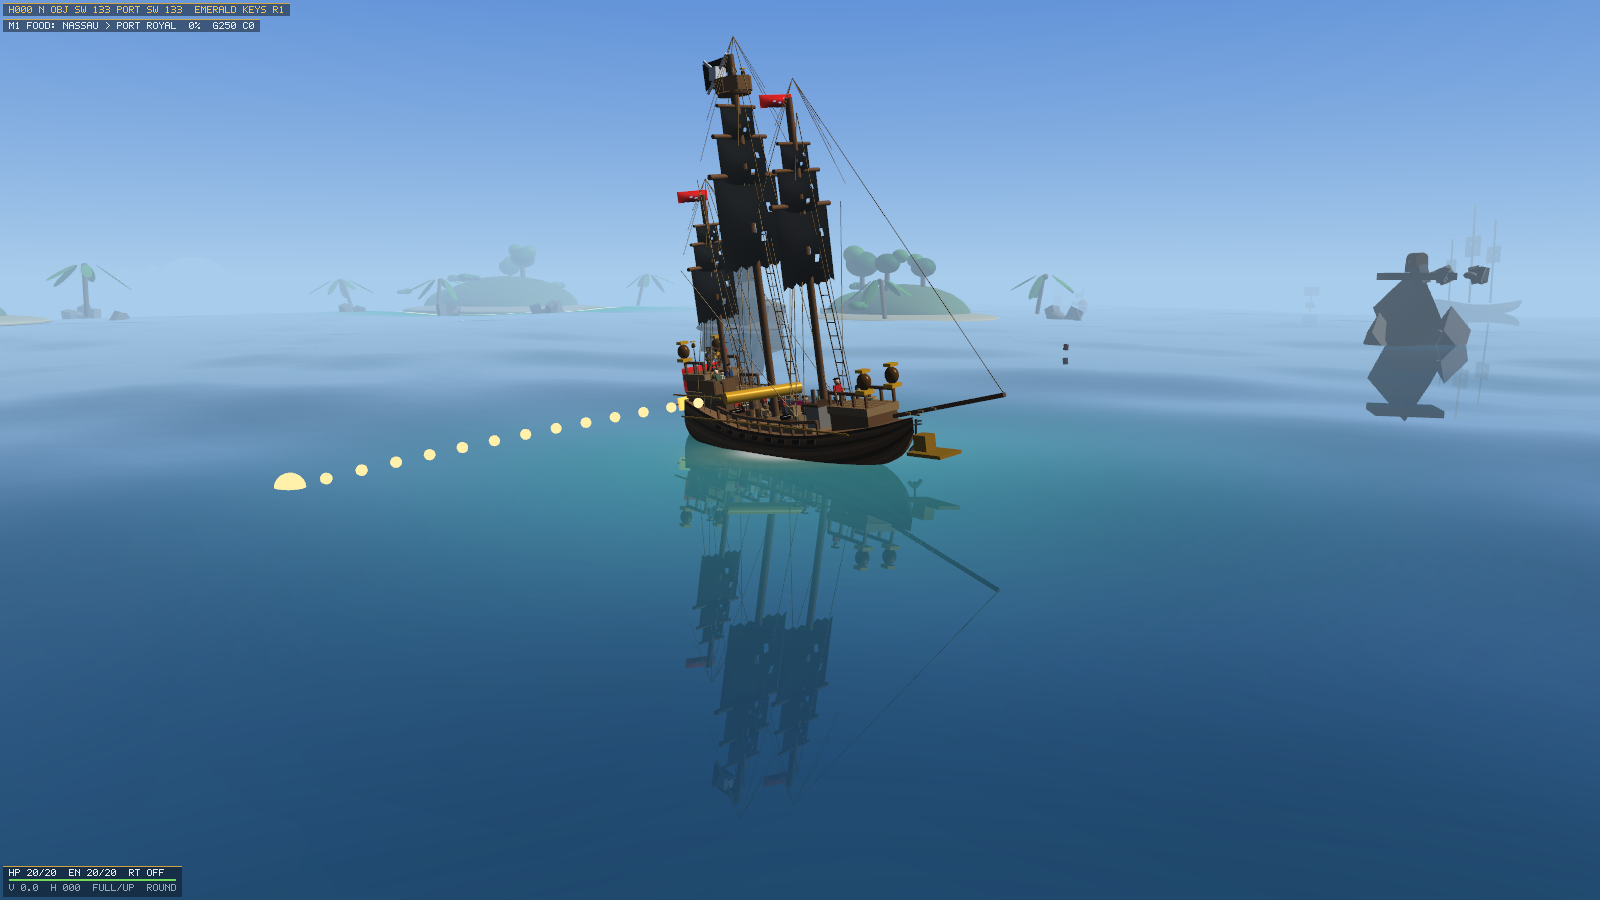
\includegraphics[width=0.31\textwidth]{figures/time_day.png} &
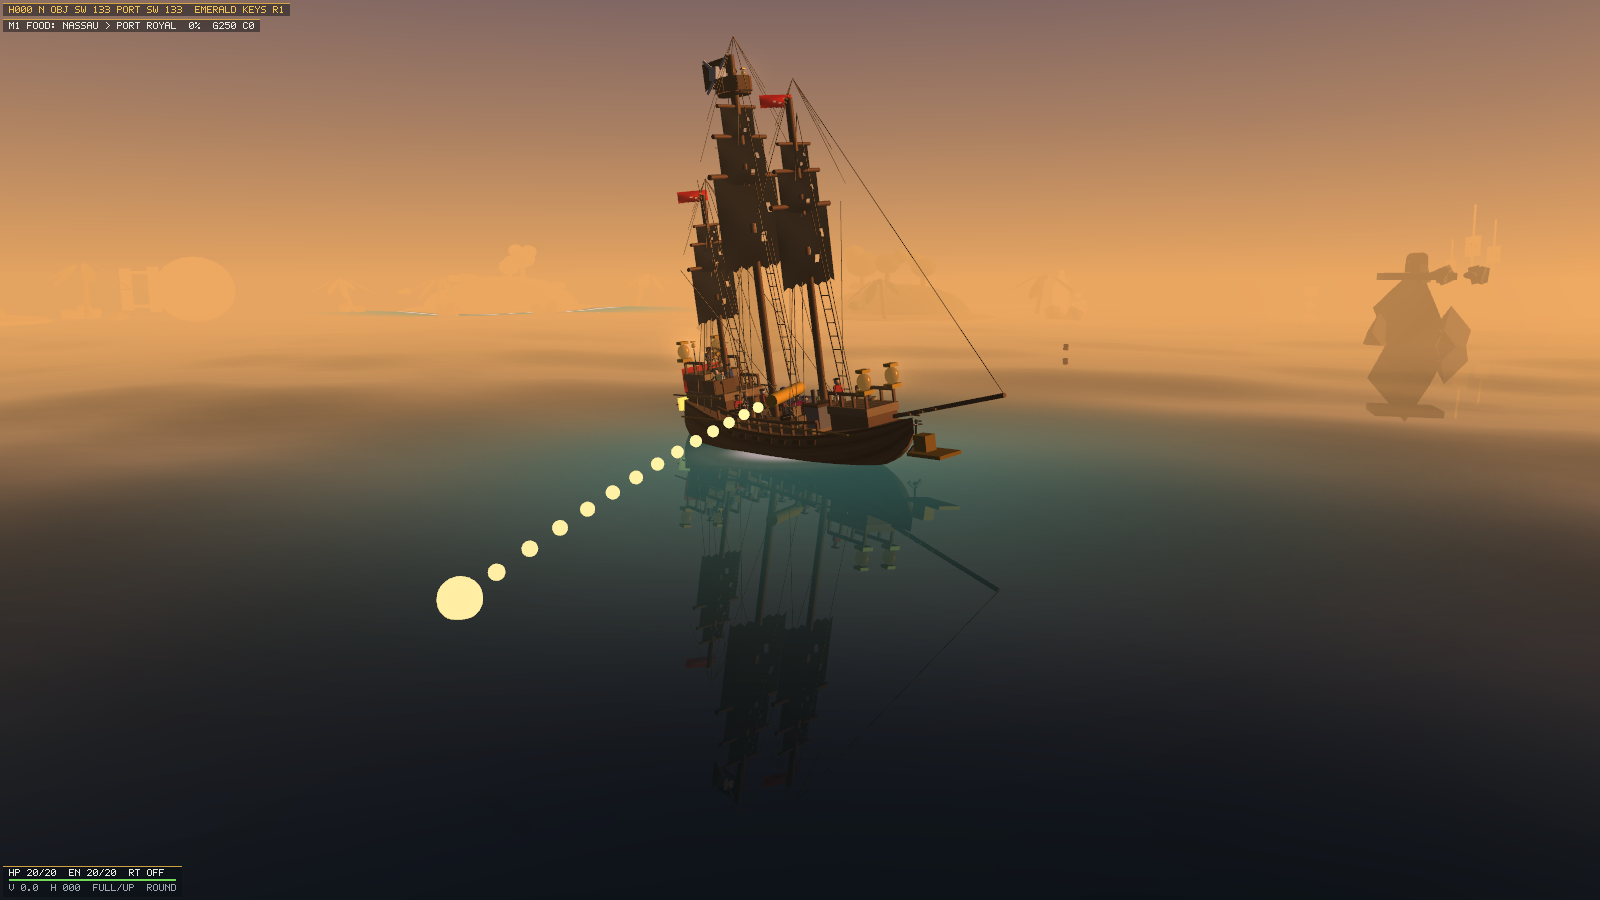
\includegraphics[width=0.31\textwidth]{figures/time_sunset.png} &
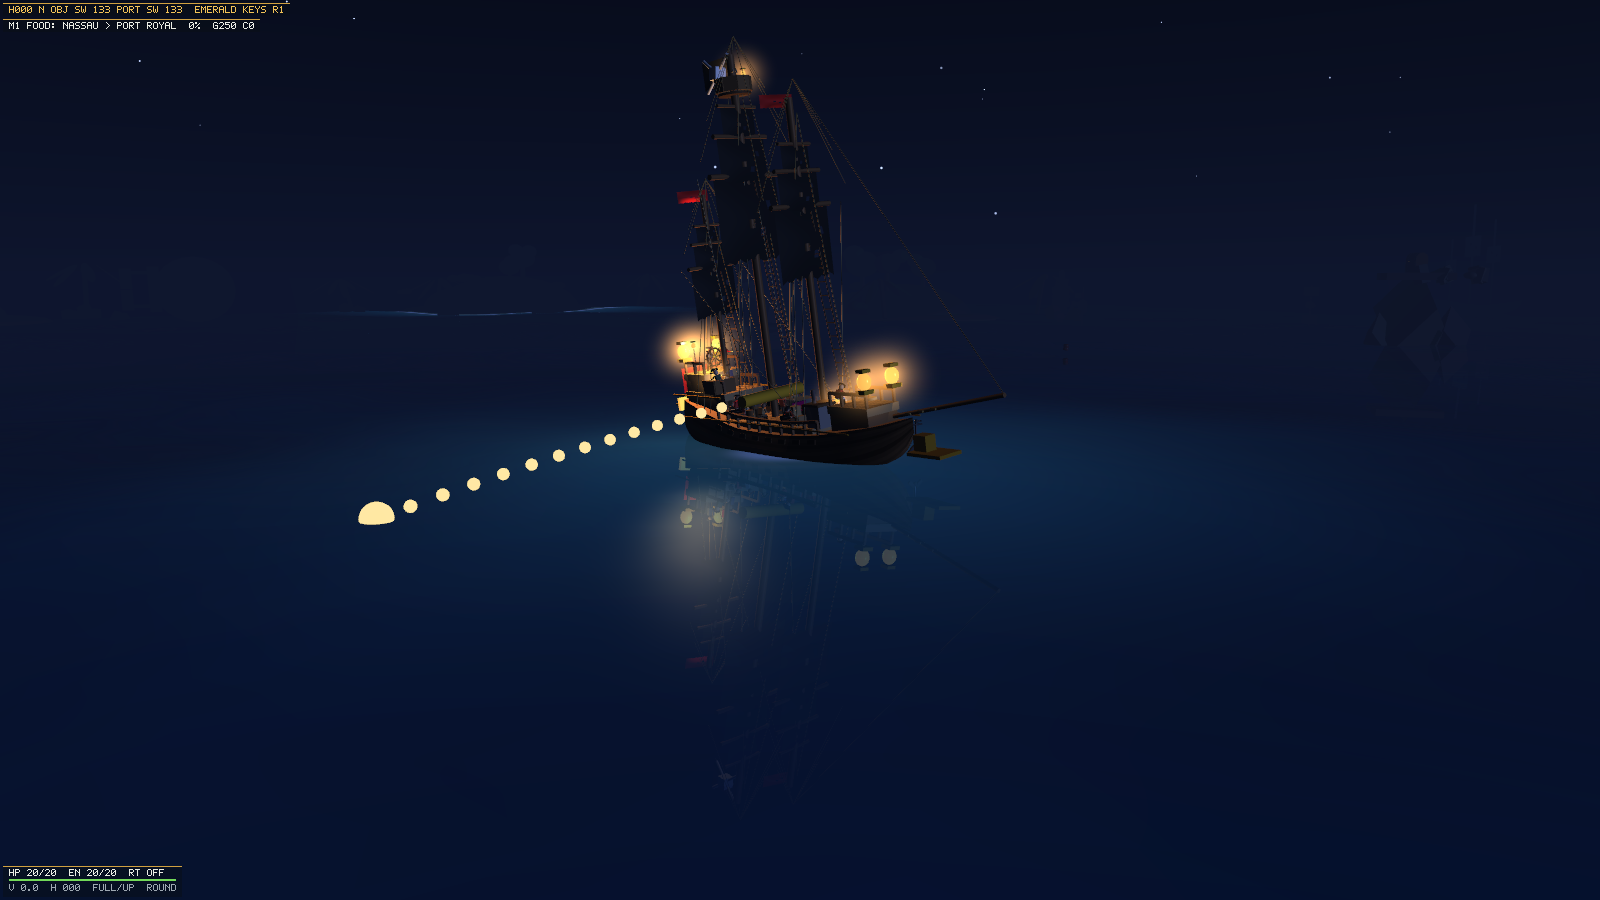
\includegraphics[width=0.31\textwidth]{figures/time_night.png} \\
\small Day & \small Sunset & \small Night \\
\end{tabular}
\caption{Time-of-day comparison with sunny weather and an unchanged camera. Night reuses the directional-light slot for moonlight and makes the emissive lantern geometry visually dominant.}
\label{fig:time-comparison}
\end{figure}

Rain quantity is bounded by \code{MAX_RAIN_DROPS=7000}. Wave amplitude is passed to both the GLSL sea displacement and the CPU ship-riding calculation. The displayed ocean and the hull motion therefore respond to the same sea state instead of behaving as unrelated animations.

% ============================================================
% CHAPTER 3
% ============================================================
\chapter{Implementation}

\section{Program Structure and Animation}
The main scene stores the player ship, enemy ships, camera, environment, particles, crew, missions, world objects, and interface settings. Other modules handle specific tasks such as waves, ships, particles, wildlife, and mission logic.

Each frame follows five steps:
\begin{enumerate}
    \item Read keyboard and mouse input.
    \item Calculate the time passed since the last frame.
    \item Update ships, water, projectiles, particles, weather, missions, and world objects.
    \item Render the updated scene.
    \item Display the frame and repeat.
\end{enumerate}

Movement uses frame time \(\Delta t\), so the simulation behaves more consistently when the frame rate changes.

The measured frame interval is clamped to \(0.10\) seconds before simulation. This prevents a paused debugger or dragged window from producing one abnormally large physics step. Many smooth controls use exponential approach,
\begin{equation}
x_{t+\Delta t}=x_t+(x_{target}-x_t)\left(1-e^{-k\Delta t}\right),
\end{equation}
which is used for effects such as steering, docking alignment, and camera transitions. Periodic motion such as waves, flags, birds, and environmental cycles is calculated as a closed function of time, avoiding stored frame-by-frame animation clips.

\section{Ship, Combat, and Particles}
The ship is built as a hierarchy. The body is the parent object, while decks, masts, sails, cannons, and crew are placed relative to it. This keeps all parts in the correct position when the ship moves, turns, pitches, or rolls.

Cannonballs use simple projectile motion:
\begin{equation}
\mathbf{p}_{new}=\mathbf{p}+\mathbf{v}\Delta t,
\end{equation}
\begin{equation}
\mathbf{v}_{new}=\mathbf{v}+\mathbf{g}\Delta t,
\end{equation}
where \(\mathbf{p}\) is position, \(\mathbf{v}\) is velocity, and \(\mathbf{g}\) is gravity. The program checks for impacts with water, land, ships, and other valid targets. Hits can create splashes, smoke, sparks, debris, or visible damage.

Particles are used for smoke, fire, sparks, splashes, foam, bubbles, and rain. A fixed maximum number of particles prevents the system from growing without limit.

For a particle with position \(\mathbf{p}\), velocity \(\mathbf{v}\), acceleration \(\mathbf{a}\), and age \(\tau\), the update follows the same explicit time integration used by projectiles:
\begin{equation}
\mathbf{v}\leftarrow\mathbf{v}+\mathbf{a}\Delta t,\qquad
\mathbf{p}\leftarrow\mathbf{p}+\mathbf{v}\Delta t,\qquad
\tau\leftarrow\tau+\Delta t.
\end{equation}
Smoke additionally receives wind drift and expands while its alpha decreases with normalized lifetime. \code{ParticleSystem} reserves a maximum of 3200 live entries and removes an expired entry by swapping it with the last live element, giving constant-time cleanup without shifting the remainder of the array.

\placeholderfigure{figures/combat.png}{Ship combat with cannon fire and particle effects.}{fig:combat}

\clearpage
\section{Below-Deck Interior and Local Lighting}
The ship is explorable rather than being only an exterior model. \code{Interior.h} builds five connected hold rooms---captain's cabin, crew quarters, cargo hold, galley, and powder magazine---in hull-local coordinates. It also defines furniture, bulkhead colliders, ladders, hatches, chests, sleepers, a cook, and lantern positions. The room boundaries query the same hull-section profile used by the exterior, so the walkable width narrows with the procedural hull.

\begin{figure}[H]
\centering
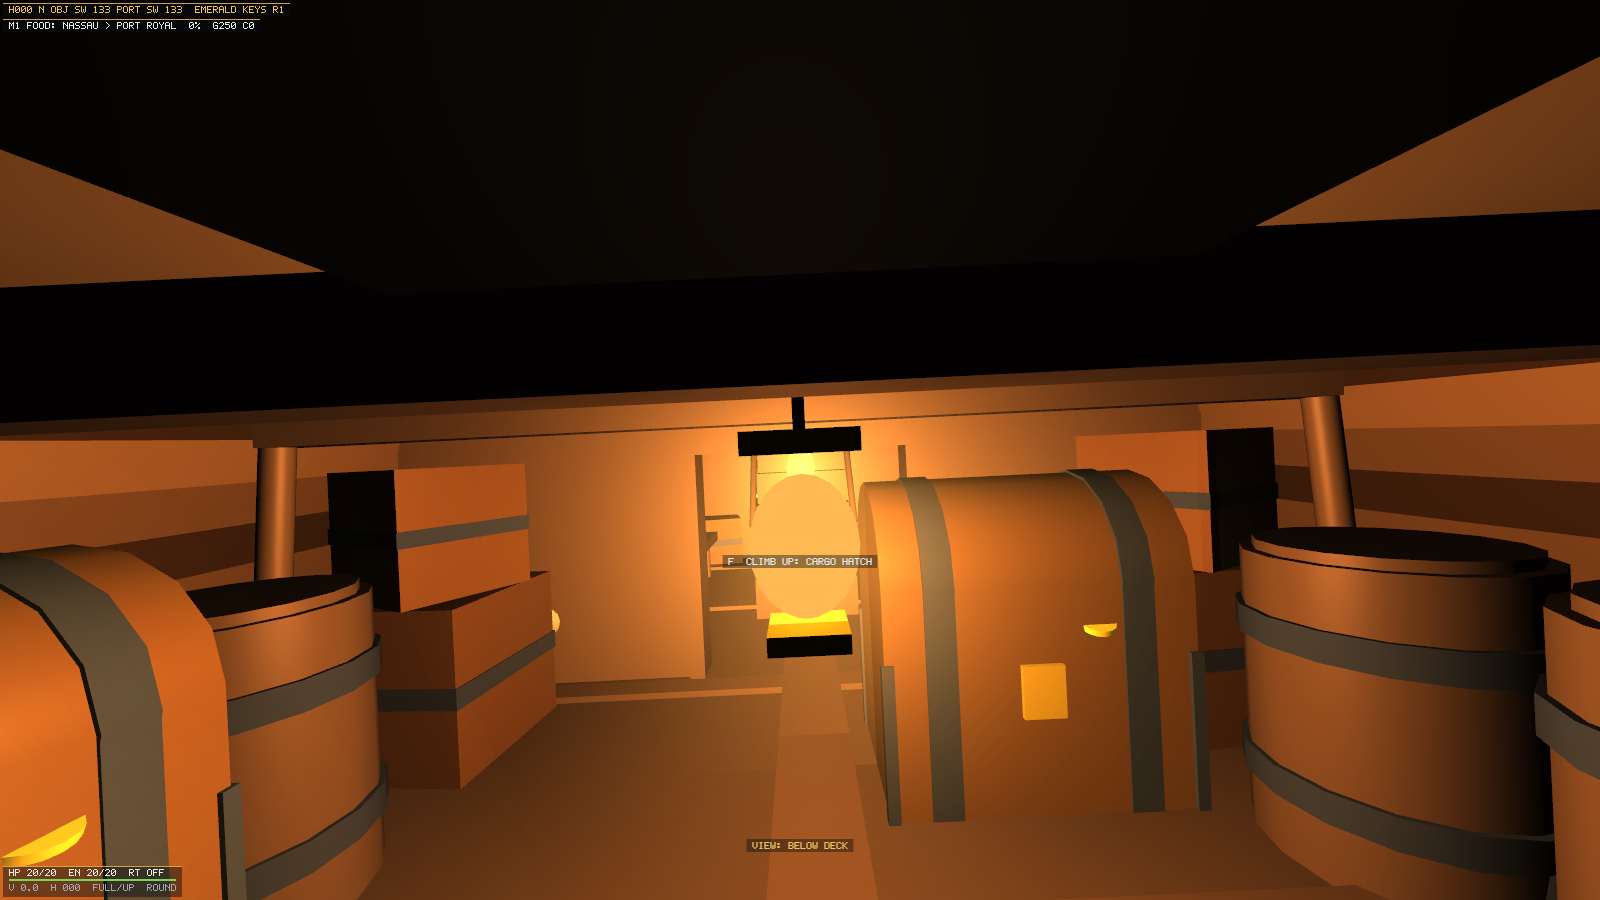
\includegraphics[width=0.75\textwidth]{figures/inside_deck_cargo.png}
\caption{Cargo hold rendered from the below-deck first-person camera. Crates, barrels, a chest, hull frames, roof beams, and the cargo-hatch ladder are procedurally placed.}
\label{fig:interior-cargo}
\end{figure}

\begin{figure}[H]
\centering
\begin{tabular}{cc}
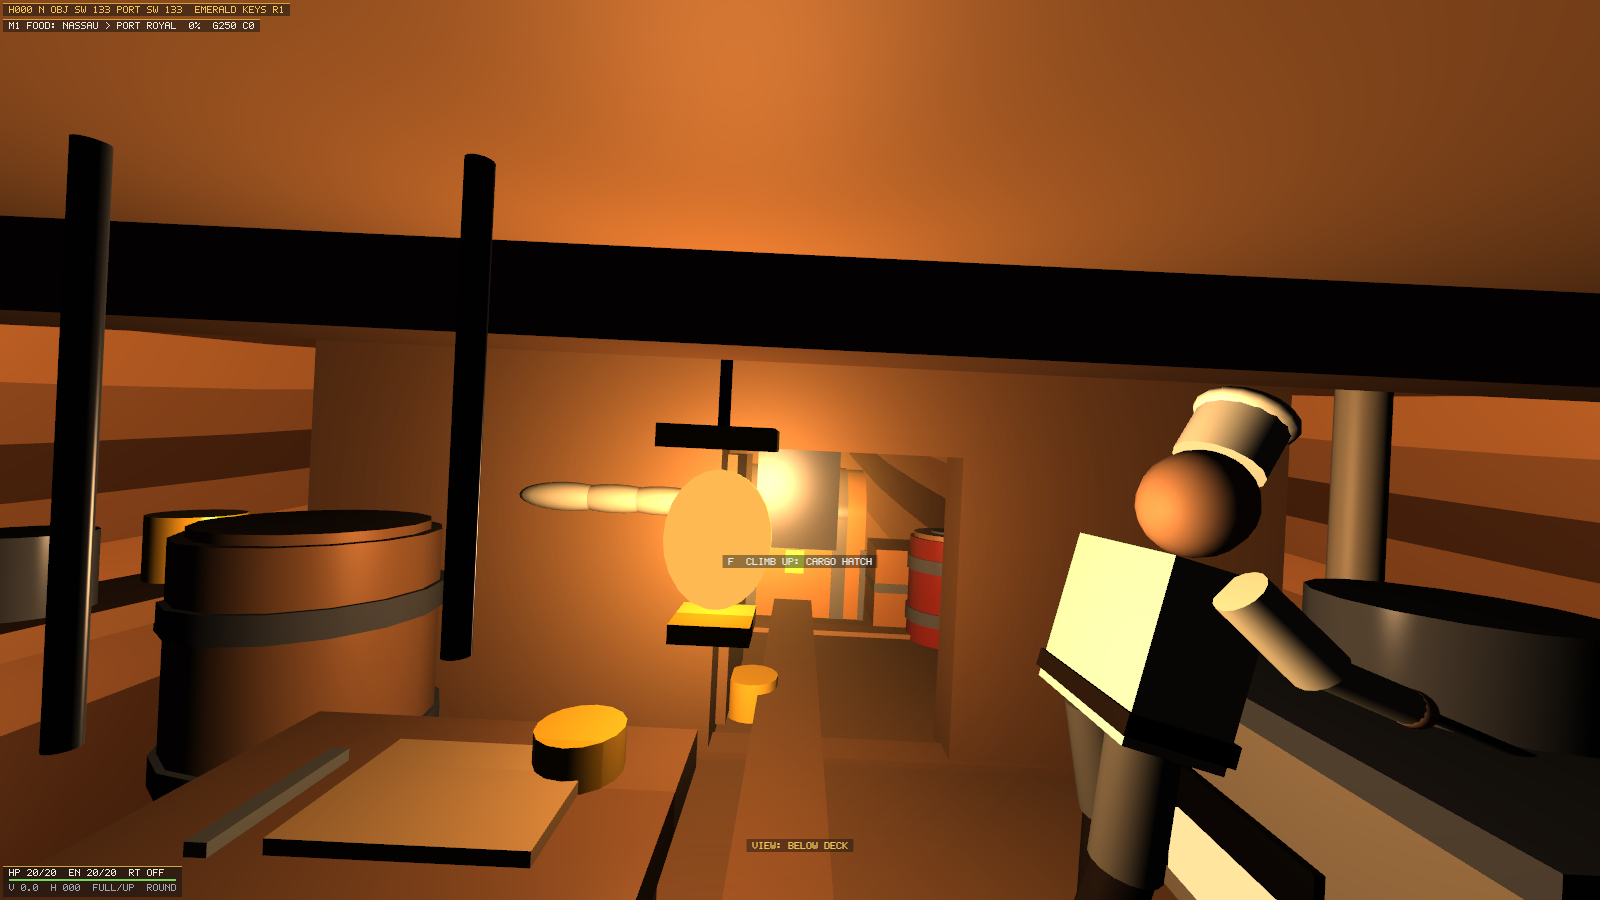
\includegraphics[width=0.46\textwidth]{figures/inside_deck_galley.png} &
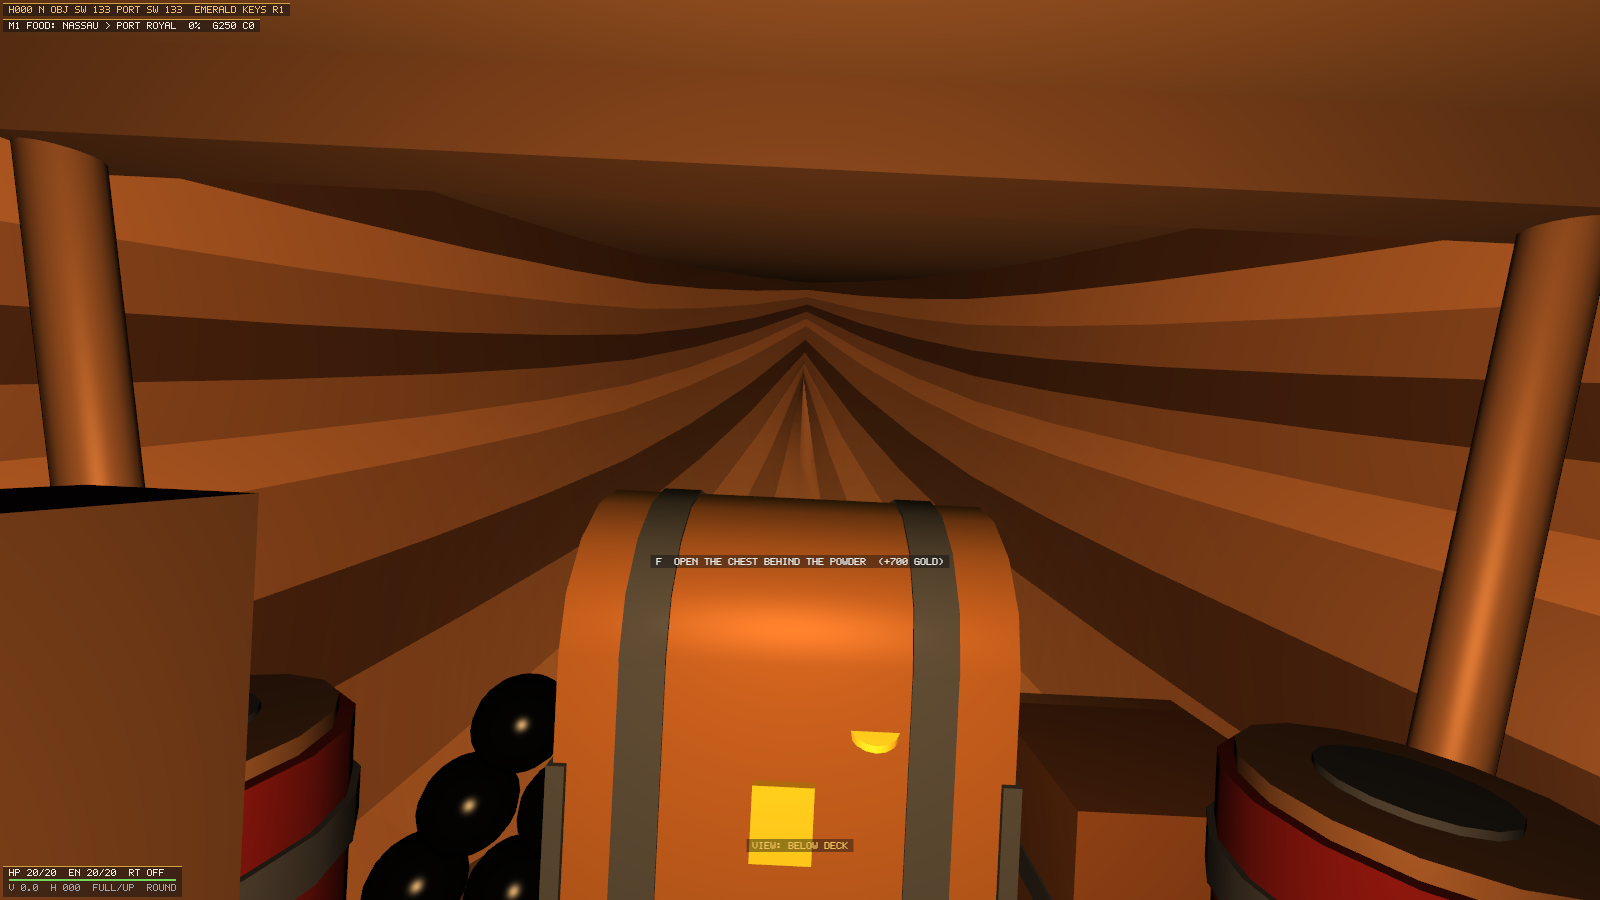
\includegraphics[width=0.46\textwidth]{figures/inside_deck_magazine.png} \\
\small Galley and cook & \small Powder magazine and protected chest \\
\end{tabular}
\caption{Two further interior states. The scene keeps a low warm ambient term and lends the existing point-light slot to the lantern nearest the explorer.}
\label{fig:interior-rooms}
\end{figure}

When the camera is inside, the outside sky, sea, weather, and ships are skipped. The hull shell is viewed from within by reversing culling and flipping its normals for the draw, after which the normal state is restored. Sun colour is set to zero, haze is disabled, and warm ambient plus the nearest lantern illuminate the room. This is a separate rendering state, not an unrelated model or a pre-rendered backdrop. \code{TAB} enters/leaves exploration, \code{WASD} moves, mouse motion looks around, and \code{F} uses a nearby ladder, hatch, or chest.

\section{World, Missions, and Navigation}
The world includes ports, trade goods, missions, crew activity, wildlife, and moving vessels. A ship can approach a port, dock, trade, and continue to another location. Missions include activities such as delivery, escort, rescue, treasure recovery, and combat. The navigation system can show useful targets and distances.

\code{Campaign.h} defines 13 ports, 14 cargo types, a 24-unit hold, timed cargo transfers, supply/demand prices, port relationships, state-based dock approach, port NPC work routes, treasure-map uncertainty, and ten connected missions. The mission sequence covers delivery, escort, trade, rescue, storm survival, treasure recovery, raid, named-captain hunt, port defence, and escape. Success grants the stored reward once and advances to the next definition; failure restarts the current mission after its result timer.

\code{LivingWorld.h} adds eight outer regions and persistent discoveries. Traffic follows routes associated with faction and region instead of choosing an unrelated random direction every frame. An encounter manager considers location, distance, weather, time, reputation, and mission context. Nearby land and vessel checks are spatially bounded so remote world content does not receive the full rendering and interaction cost.

\begin{figure}[H]
\centering
\begin{tabular}{cc}
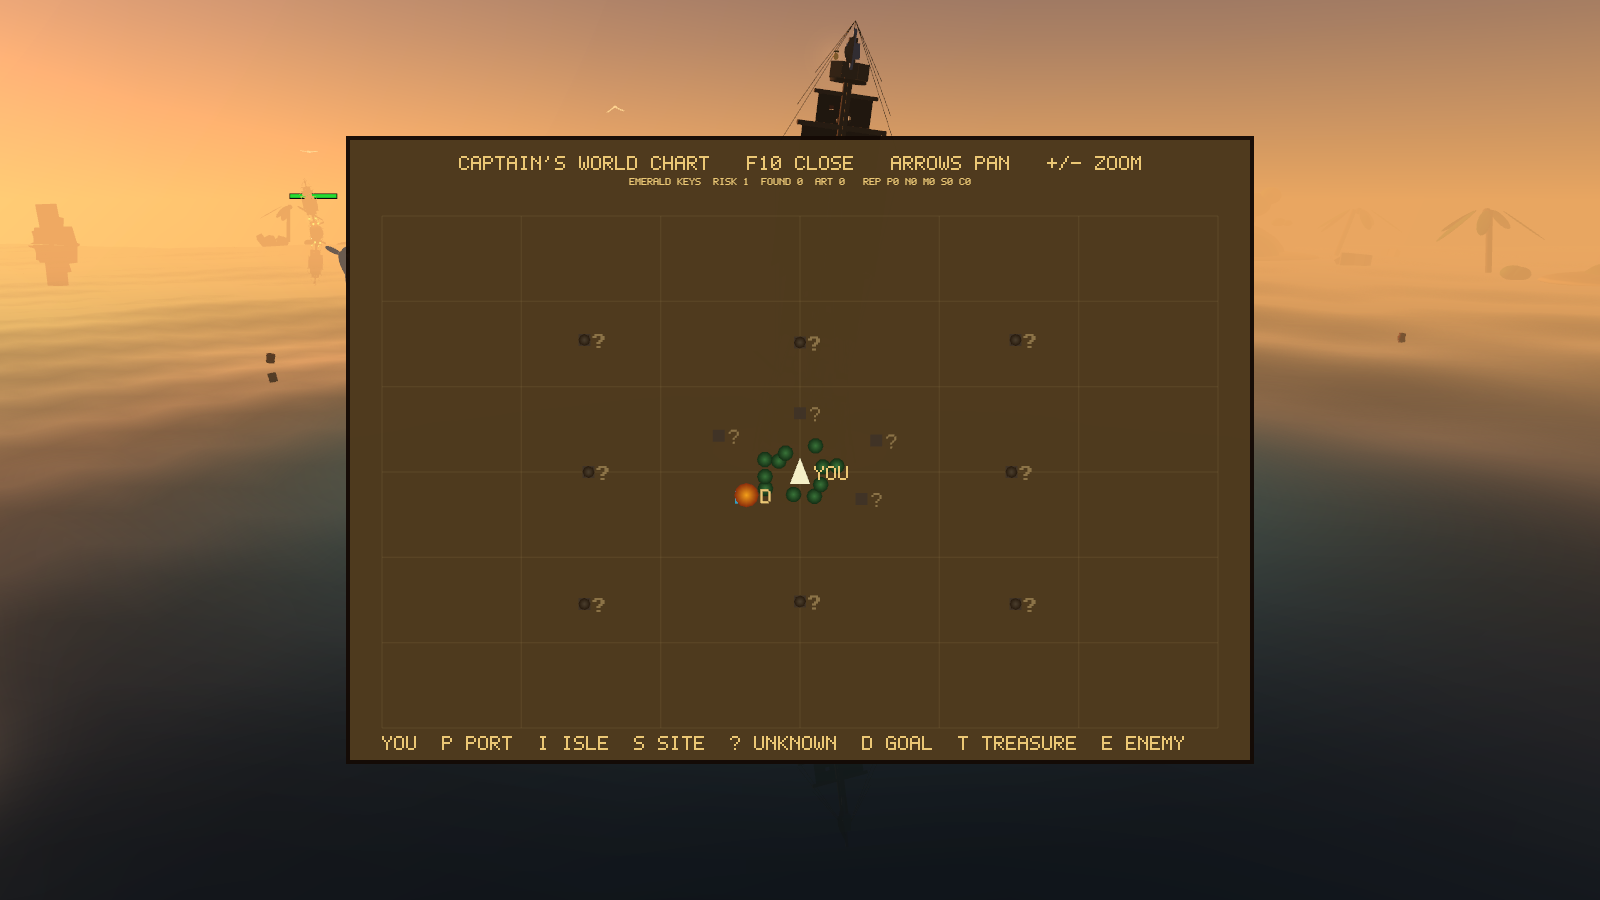
\includegraphics[width=0.46\textwidth]{figures/world_map.png} &
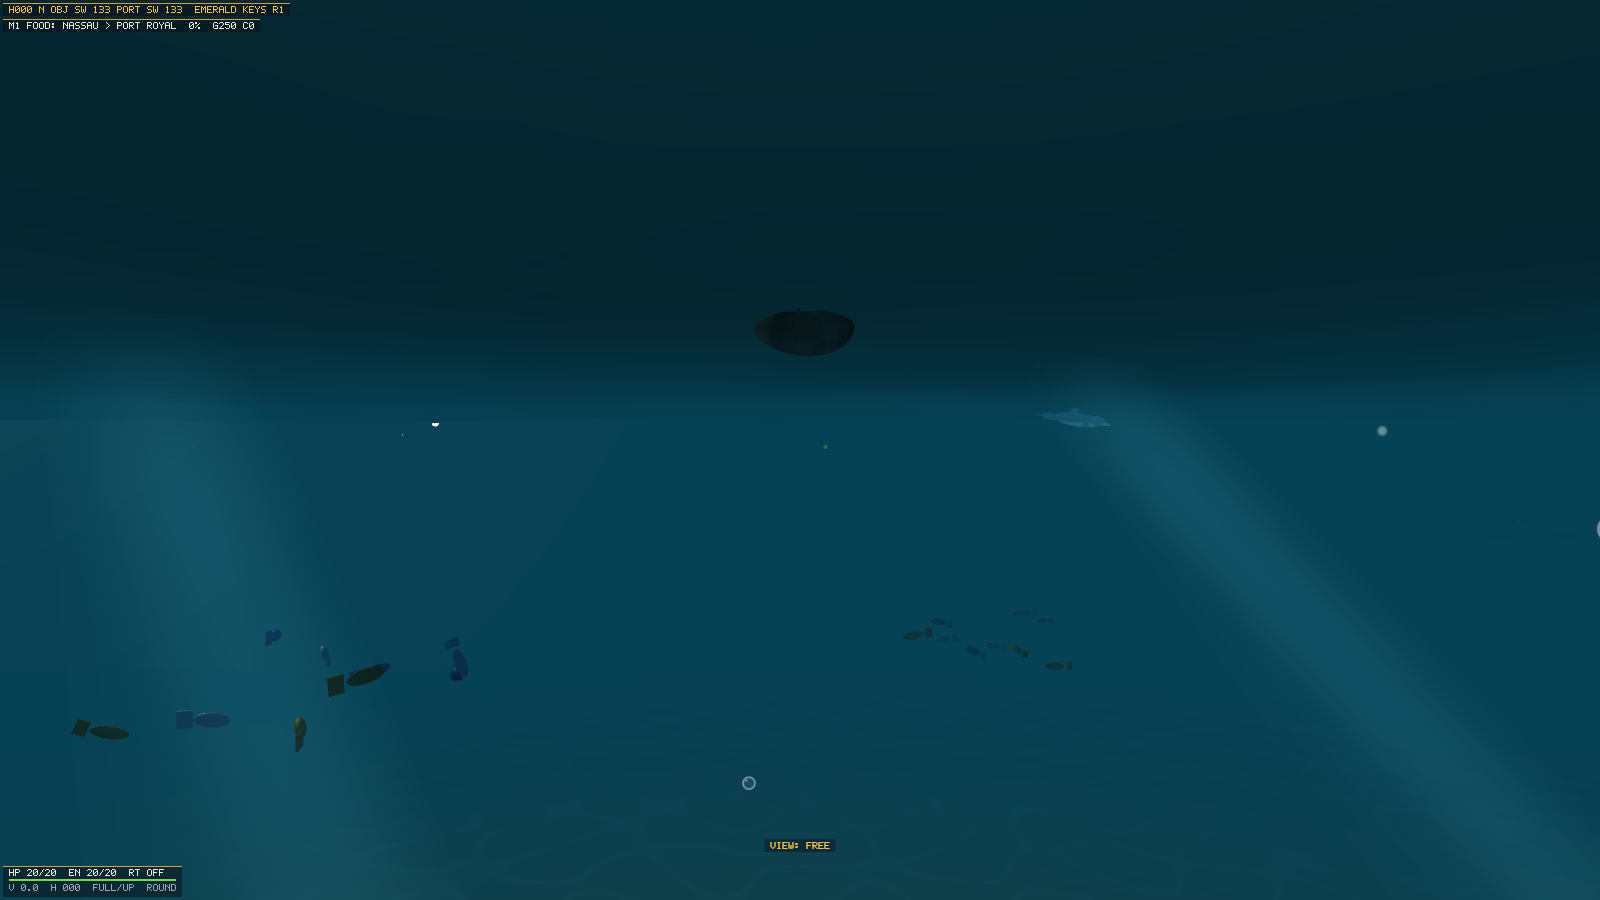
\includegraphics[width=0.46\textwidth]{figures/underwater_scene.png} \\
\small Interactive world chart & \small Underwater rendering state \\
\end{tabular}
\caption{Exploration systems beyond the original proposal. The chart shows navigation state; the underwater view changes haze, surface appearance, caustics, particles, vegetation, fish, and visibility.}
\label{fig:exploration-systems}
\end{figure}

These systems are simpler than those in a full commercial game. Their purpose is to connect the graphics demonstrations into a navigable world while retaining bounded, inspectable state machines.

\section{User Interaction}
GLFW reads the keyboard, mouse, mouse buttons, and scroll wheel \cite{glfw}. The main controls are summarized below.

\begin{table}[H]
\centering
\caption{Important controls in the simulation.}
\label{tab:controls}
\small
\begin{tabularx}{0.96\textwidth}{p{0.20\textwidth}p{0.29\textwidth}Y}
\toprule
\textbf{Input} & \textbf{Purpose} & \textbf{Effect} \\
\midrule
WASD / arrows & Ship movement & Apply forward/reverse thrust and steering; steering drives the helm, wheel, and rudder. \\
Mouse; Space / right click & Aiming and fire & Mouse position chooses aim; the fire input launches one shot subject to reload. \\
Ctrl; Y & Broadside / ammunition & Fire the battery toward the enemy; cycle round, chain, and grape shot. \\
Z; J & Sails / anchor & Cycle full, half, and furled sails; lower or raise the animated anchor. \\
F1--F5; R & Prepared cameras & Glide to five orbit presets; reset to the first preset. \\
F6--F9 & Camera modes & Toggle free, first-person, cinematic, and captain views. \\
Mouse drag / scroll & Camera movement & Rotate or zoom supported views. \\
TAB; F & Exploration & Enter the deck/interior or go ashore; use ladders, hatches, chests, trade, and nearby interactions. \\
F10; arrows; +/- & World chart & Open the chart, pan it, and adjust its zoom. \\
I, C, T & Environment & Cycle location, weather, and time settings; Shift reverses the cycle. \\
Esc; Backspace & Interface & Pause/open options; independently show or hide the compact HUD. \\
0 & Hybrid ray tracing & Toggle ray-tested direct-sun visibility on the ocean. \\
1, 2, 3 & Shading & Select Flat, Gouraud, or Phong shading. \\
K, B, L & Lighting & Cycle lighting terms, Phong/Blinn specular, and light masks. \\
\bottomrule
\end{tabularx}
\end{table}

\clearpage
\section{Hybrid Ray-Traced Sun Shadows on the Ocean}
The scene remains a normal OpenGL rasterizer. The additional feature is genuine but deliberately narrow: every above-water ocean fragment may cast one analytic ray toward the existing directional sun. The ray is tested against at most 16 bounding spheres representing nearby ship hull sections, intact mast/sail stacks, world vessels, islands, rocks, and surface sites. This follows the standard ray--sphere test while avoiding triangle traversal, compute shaders, RTX APIs, external libraries, and acceleration structures \cite{pbrt}.

For water position \(\mathbf{P}\), interpolated wave normal \(\mathbf{N}\), and normalized direction \(\mathbf{D}\) toward the sun, the biased ray is
\begin{equation}
\mathbf{R}(t)=\mathbf{O}+t\mathbf{D},\qquad
\mathbf{O}=\mathbf{P}+0.05\mathbf{N}.
\end{equation}
For a proxy sphere with centre \(\mathbf{C}\) and radius \(r\), the fragment shader evaluates
\begin{align}
\mathbf{o}_c &= \mathbf{O}-\mathbf{C},\\
b &= \mathbf{o}_c\cdot\mathbf{D},\\
c &= \mathbf{o}_c\cdot\mathbf{o}_c-r^2,\\
h &= b^2-c,\\
t_{near} &= -b-\sqrt{h}.
\end{align}
A forward intersection exists when \(h\geq0\) and a root exceeds the \(0.08\) epsilon. The reusable GLSL function \code{rayIntersectsSphere} performs this test; \code{isSunBlocked} loops over \code{uRaySpheres[16]}. The CPU function \code{buildRayTraceProxies} reads current world-space ship frames and scenery positions, filters candidates to a 190-unit range, sorts them by camera distance, and uploads the closest 16 as \((C_x,C_y,C_z,r)\). Broken masts are omitted, while moving hull and vessel proxies are rebuilt from their current frames every rendered frame.

The result is a binary visibility value \(V_s\). The existing Phong terms are still evaluated, but only direct directional-light terms are gated:
\begin{equation}
\mathbf{I}=\mathbf{I}_a+V_s(\mathbf{I}_{d,sun}+\mathbf{I}_{s,sun})
+\mathbf{I}_{point}+\mathbf{k}_e,
\qquad
V_s=\begin{cases}0,&\text{blocked},\\1,&\text{visible}.\end{cases}
\end{equation}
Ambient light, the local point light, emission, haze, foam, shallows, and the rasterized planar reflection remain active. Consequently a ray-shadowed ocean region is visibly darker but not black. With the toggle off, \code{gSunVisibility} stays exactly \(1\), preserving the original Phong path.

\begin{figure}[H]
\centering
\begin{tabular}{cc}
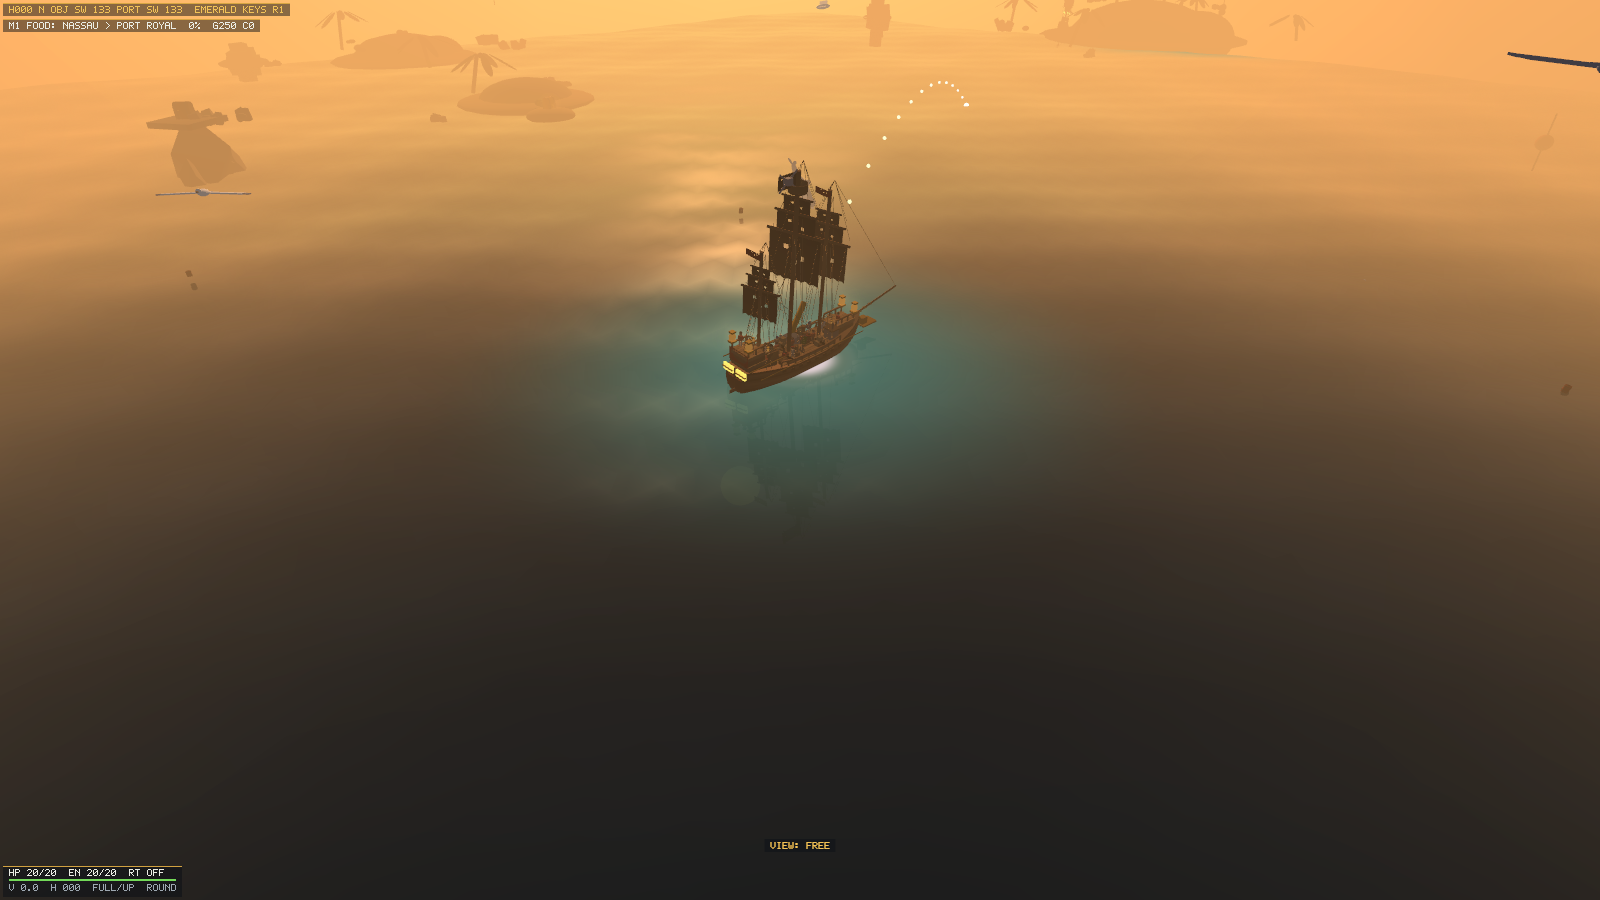
\includegraphics[width=0.47\textwidth]{figures/ray_tracing_off.png} &
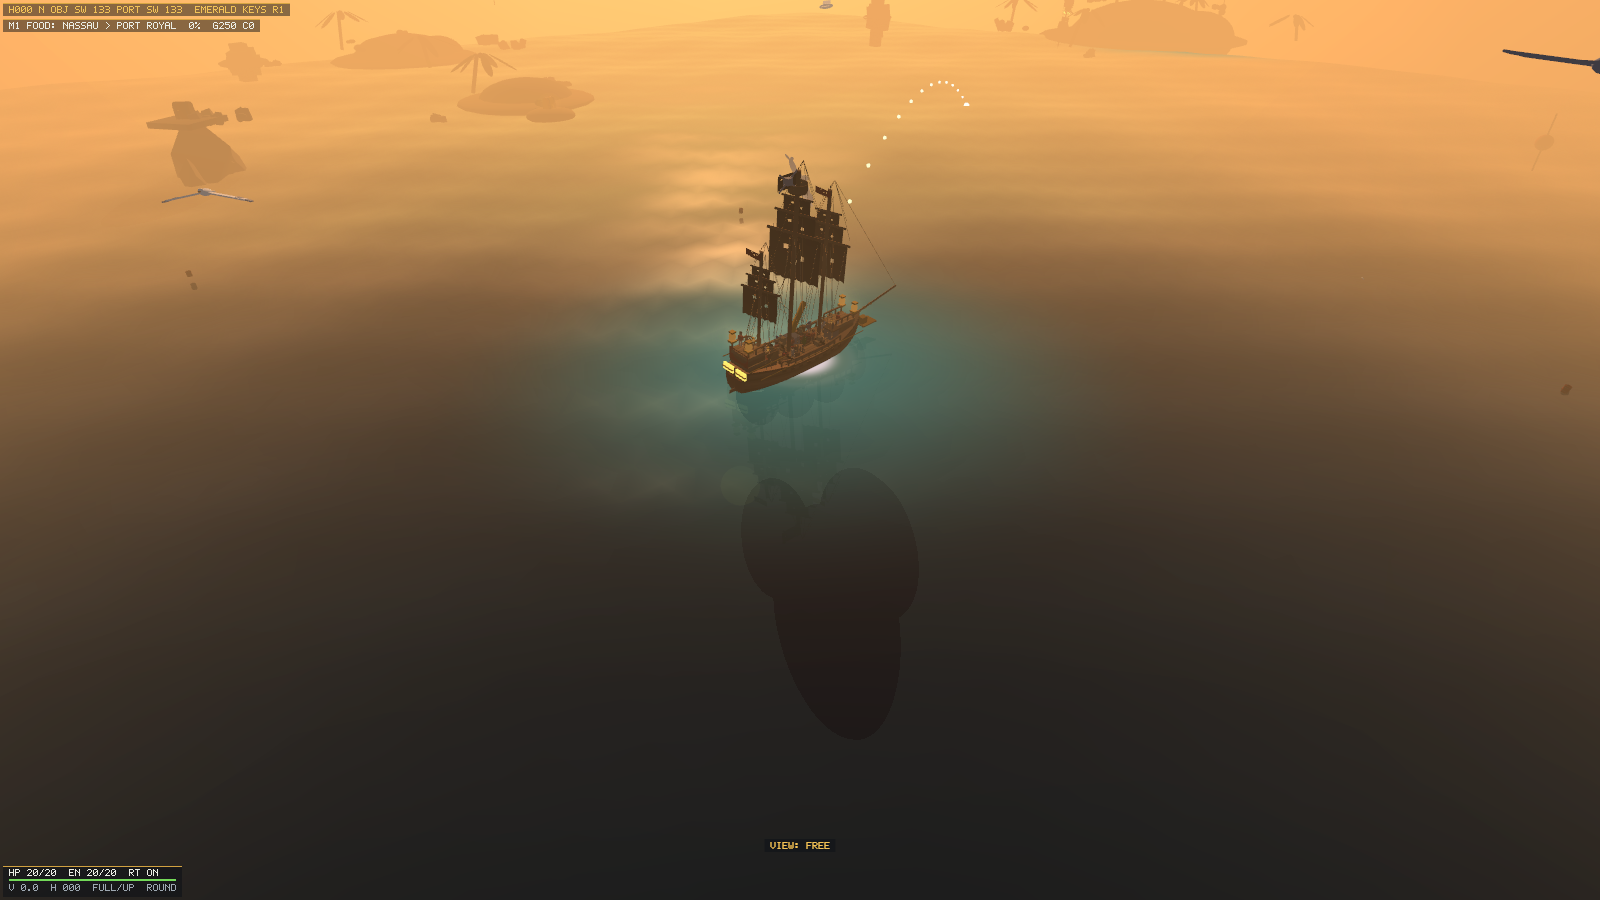
\includegraphics[width=0.47\textwidth]{figures/ray_tracing_on.png} \\
\small Ray tracing OFF: rasterized baseline & \small Ray tracing ON: proxy shadow on the ocean \\
\end{tabular}
\caption{Matched sunset camera comparison. The ON image contains the long dark ocean shadow cast away from the directional sun by the current hull and mast proxy spheres; the HUD also changes from RT OFF to RT ON.}
\label{fig:ray-comparison}
\end{figure}

The \code{0} key is edge detected: one press flips \code{SceneState::rayTracingEnabled} once, updates the compact HUD immediately, and uploads \code{uRayTracingEnabled} for the water draw. The command-line \code{--raytrace} option initializes the same state for reproducible screenshots. The limitation is visible in the shadow boundary: it represents analytic spheres rather than the exact sails and rigging, and it produces hard visibility rather than multi-sample soft shadows. The existing planar water reflection is rasterized and is not described as ray tracing.

% ============================================================
% CHAPTER 4
% ============================================================
\chapter{Results and Discussion}

\section{Main Results}
The final program meets the main graphics goals and adds several extra features. Table~\ref{tab:requirements} gives a short comparison.

\begin{table}[H]
\centering
\caption{Main project goals and final results.}
\label{tab:requirements}
\small
\begin{tabularx}{0.97\textwidth}{p{0.27\textwidth}p{0.15\textwidth}Y}
\toprule
\textbf{Goal} & \textbf{Status} & \textbf{Final result} \\
\midrule
Sea surface & Extended & Animated waves, foam, shallow-water effects, and underwater viewing. \\
Multiple ships & Extended & Player, enemies, and other vessels. \\
Cannons & Implemented & Aiming, firing, projectile motion, and impact effects. \\
Sky and environment & Extended & Day/night settings, weather, haze, rain, and lighting changes. \\
Lighting & Implemented & Ambient, diffuse, and specular terms. \\
Phong shading & Implemented & Per-fragment Phong shading is available. \\
Transformations & Implemented & Translation, rotation, scaling, camera matrices, and ship hierarchy. \\
Animation & Extended & Water, ships, projectiles, crew, particles, wildlife, and weather. \\
Interaction & Extended & Sailing, firing, camera, map, HUD, and graphics controls. \\
Hybrid ray tracing & Extra & Per-fragment ocean-to-sun rays test up to 16 animated world-space proxy spheres. \\
\bottomrule
\end{tabularx}
\end{table}

\section{Visual Results and Performance}
The project provides clearly different scenes for showing the graphics concepts. Daytime scenes show the ship, sea, lighting, and camera. Storm scenes show weather changes. Combat scenes show projectile and particle animation. Gouraud and Phong screenshots allow the two shading methods to be compared using the same scene. The matched ray-shadow screenshots show the hybrid visibility result from the same camera.

Several design choices help the program remain suitable for real-time rendering. Basic meshes are reused, particles have a fixed limit, distant objects can be simplified or skipped, and the hybrid ray pass checks only a small number of simplified objects. The program also includes draw and geometry counters that can help inspect rendering workload.

\begin{table}[H]
\centering
\caption{Bounded resources and important demonstration parameters.}
\label{tab:limits}
\small
\begin{tabularx}{0.92\textwidth}{p{0.28\textwidth}p{0.16\textwidth}Y}
\toprule
\textbf{Parameter} & \textbf{Value} & \textbf{Effect of changing it} \\
\midrule
\code{ParticleConfig::CAPACITY} & 3200 & Bounds simultaneous smoke, fire, sparks, splash, foam, bubbles, and related particles. \\
\code{EnvironmentConfig::MAX_RAIN_DROPS} & 7000 & Caps generated rain line segments at maximum rain intensity. \\
\code{PlayConfig::MAX_BALLS} & 96 & Bounds simultaneous reusable cannonball slots. \\
\code{RayTraceConfig::MAX_SPHERES} & 16 & Sets the maximum ray--sphere intersection tests per ocean fragment. \\
\code{RayTraceConfig::PROXY_RANGE} & 190 units & Excludes distant occluders that cannot usefully affect the nearby visible demonstration. \\
Damage pools & 10 fires, 14 holes, 24 rails, 96 debris & Prevents progressive damage and temporary effects from growing without limit. \\
Cargo capacity & 24 units & Constrains trading choices and visible/timed cargo operations. \\
Frame-time clamp & 0.10 s & Prevents a delayed frame from advancing animation or collision by an unsafe step. \\
\bottomrule
\end{tabularx}
\end{table}

Mesh reuse separates stored geometry from submitted draws: the same cube, cylinder, sphere, sail, and other generated meshes are transformed into many objects. A distance check precedes many distant-world, particle, wildlife, and proxy operations. Static cannon-port and carriage parts also have an optional merged submission path. The living world uses simplified geometry for distant traffic and renders nearby detail only where it can contribute to the current frame.

A fixed FPS value is not reported because it depends on the computer, resolution, camera position, and graphics settings. A proper benchmark should state these conditions.

\section{Testing, Challenges, and Limitations}
The project includes command-line checks for important program states and camera behavior. These tests help verify logic, but the final visual result must still be checked by running the OpenGL window.

The integrated CPU test currently performs 31 checks. Relevant results include forward ray hit versus miss/behind-ray classification, ten connected mission definitions, bounded cargo capacity, timed loading, automatic docking, compass updates, deterministic archipelago generation, minimum encounter distance, persistent discoveries, dolphin continuity, and enemy routing through ports and narrow passages. The Release configuration builds successfully and both GLSL programs report successful links at runtime. Matched 1600\(\times\)900 screenshots verify that the ray toggle changes the ocean while the normal scene, Phong shading, animation, interaction, and planar reflection remain operational.

The main implementation challenge was keeping the systems consistent. For example, the ship uses the same wave idea as the rendered water, and the lighting model is kept similar when comparing Gouraud and Phong shading. The ship hierarchy also makes sure child objects move correctly with the ship.

The main limitations are:
\begin{itemize}
    \item Some objects use simple procedural models instead of highly detailed assets.
    \item Port and cargo activities use simple state-based logic instead of full physical simulation.
    \item The ray-based ocean shadow uses simplified sphere shapes instead of exact object triangles.
    \item In Gouraud mode with ray tracing enabled, the ocean alone re-evaluates shared lighting per fragment so a fragment-level visibility ray can affect it; the normal RT-off Gouraud demonstration remains unchanged.
    \item The project does not implement complete physically based rendering or full ray tracing.
\end{itemize}

These limits are acceptable because the main purpose is to demonstrate computer graphics concepts clearly.

% ============================================================
% CHAPTER 5
% ============================================================
\chapter{Conclusion and Future Work}

\section{Conclusion}
The \emph{3D Ship Battle Simulation Using OpenGL} combines the main graphics topics needed for an interactive 3D course project. It uses direct OpenGL rendering, reusable geometry, model-view-projection transformations, multiple shading methods, ambient-diffuse-specular lighting, animated water, projectile motion, particles, camera control, and user interaction.

The project also adds weather, ports, missions, wildlife, crew, navigation, and other world activity. These extra features provide more situations where the graphics techniques can be seen. The user can switch shading modes, move the camera, sail the ship, fire cannons, change the environment, and compare effects while the program is running.

\section{Future Work}
Possible improvements are:
\begin{itemize}
    \item more detailed ship and environment models;
    \item more accurate collision shapes;
    \item improved water reflections and shadows;
    \item better ray intersection geometry and soft shadows;
    \item sound effects and background audio;
    \item a complete save/load system; and
    \item formal FPS testing on clearly stated hardware.
\end{itemize}

% ============================================================
% REFERENCES
% ============================================================
\renewcommand{\bibname}{References}
\small
\bibliographystyle{IEEEtran}
\bibliography{references}

\end{document}
